\documentclass[11pt]{article}
\usepackage[preprint]{acl}
\usepackage{times}
\usepackage{latexsym}
\usepackage[T1]{fontenc}
\usepackage[utf8]{inputenc}
\usepackage{microtype}
\usepackage{graphicx}
\usepackage{booktabs}
\usepackage{amsmath,amssymb,amsthm}
\usepackage{multirow}
\usepackage{tikz}
\usetikzlibrary{arrows.meta,positioning,fit,backgrounds}
\usepackage{enumitem}

% Keep review line numbers inside the two-column gutter.
\makeatletter
\ifacl@linenumbers
  \font\aclhvsmall=phvb at 6.5pt
  \renewcommand\linenumberfont{\aclhvsmall\color{lightgray}}
  \setlength{\linenumbersep}{8pt}
\fi
\makeatother

\newtheorem{proposition}{Proposition}
\newtheorem{corollary}{Corollary}
\newcommand{\method}{FinPlan}
\newcommand{\E}{\mathbb{E}}
\newcommand{\Prob}{\mathbb{P}}
\newcommand{\indic}{\mathbf{1}}

\title{\method: A Decision Interface for Point-in-Time Financial Evidence}
\author{Anonymous ACL submission}

\begin{document}
\sloppy
\maketitle

\begin{abstract}
Financial questions about forward-looking guidance do not have a single answer at the filing date. A system can answer from the guidance midpoint, qualify the answer with a credible set, or wait for a later filing. The choice depends on later evidence and an asymmetric loss. Existing RAG and claim-verification systems fix the output mode, decision time, and budget before evidence. We formulate the output interface as a decision problem over a credal evidence state, with actions for answering, adjudicating, abstaining, acquiring evidence, and waiting. We show why point answers, relevance-only retrieval, and pre-hoc routing cannot represent the full interface. We build a year-wise company-disjoint benchmark of 273 revenue-guidance claims, with a 737-claim rolling-origin extension. On XBRL-verified labels, balanced accuracy rises from .333 to .564 and macro F1 from .220 to .488. On a non-LLM random-forest backbone, a loss-aware portfolio over fixed adjudication, abstention, and the planner matches the oracle best fixed policy in nine of ten loss configurations (regret 0) and beats it under the wide-width penalty (4.34 versus 4.71; regret -0.370, 95\% CI [-0.643, -0.100]). Mean regret is -0.037 (95\% CI [-0.064, -0.010]) with maximum 0.000; a pre-specified seed replication confirms the wide-width gain and an exact base match. Six named baselines (FinDVer, Fin-Fact, Self-RAG, CRAG, FLARE, and Adaptive-RAG), adapted under the same DeepSeek backbone, have higher selective accuracy and lower AURC than FinPlan, but lower balanced accuracy; a second backbone (GLM 5.3 flash) preserves the balanced-accuracy advantage; no point model dominates, and the decision portfolio is selected on regret. A DeepSeek-backed conformal variant is competitive in three regimes but is sensitive to masking and pretraining exposure. No fixed output interface is uniformly near-optimal; on a real earnings-release stream, a sequential portfolio matches the oracle best policy across 24 cost cells.
\end{abstract}

\section{Introduction}

Consider an analyst reading an 8-K filing on July 30. Management earnings guidance is a central disclosure channel \citep{hirst2008management}, and the company guides third-quarter revenue to \$100--110 million. The analyst must decide whether revenue will land below, within, or above that range. The 10-Q will not appear for several weeks. A point forecast of \$106 million is a bet. The statement that the outcome is likely within the range is a qualified judgment. Waiting for the 10-Q resolves the question, but consumes time. The best choice depends on the evidence available now, the evidence that will arrive, and the cost of being wrong.

Most financial question answering systems do not represent this choice. Retrieval-augmented generation (RAG) retrieves passages and returns an answer \citep{lewis2020rag,jiang2023flare,asai2024selfrag,jeong2024adaptiverag}. Claim verification returns a verdict such as supported or contradicted \citep{zhao2024findver,rangapur2025finfact}. Selective prediction returns an answer or an abstention \citep{chow1970optimum,geifman2017selective}. Recent financial RAG systems add typed evidence, period constraints, and provenance, but they keep the same output contract: an answer or a verdict is produced at a fixed cutoff with a fixed retrieval budget \citep{mansouri2026finrank,jiang2026finrate,chen2026hcrag,chi2026finsagent}. The interface is fixed before the evidence is seen. A system therefore cannot represent the case in which the first evidence supports a qualified judgment, a later filing settles the question, and the correct output mode changes in between.

We formulate the interface as a decision problem over a credal evidence state. A query or claim induces a feasible set over outcomes. Evidence arrives with an availability time, an acquisition cost, and a constraint on the feasible set. At a chosen decision time, the agent has a filtration that contains only evidence available at that time. The agent chooses among a point answer, a credible set, and an abstention, and may also acquire evidence or wait. The loss is asymmetric: overclaiming costs more than underclaiming, and an uninformative adjudication is not free. The decision time and the evidence cost are part of the objective; fixed cutoff and fixed budget are special cases, not assumptions. The policy must be measurable with respect to the filtration at the chosen time, so waiting is a costly action rather than free lookahead.

This formulation exposes a capability gap. Existing systems fix at least one of three dimensions: the output mode, the decision time, or the evidence budget. The components exist; the gap is a missing interface that lets a system decide when to decide, what evidence to acquire, and which output contract to use. Figure~\ref{fig:interface} illustrates the object. Evidence arrives over time; the planner stops with an answer or a credible set, or waits for a later filing. A router cannot express the trace because the mode is chosen after the belief update.

\begin{figure*}[t]
\centering
\begin{tikzpicture}[
  font=\footnotesize,
  >=Latex,
  box/.style={draw, rounded corners=2pt, align=center, text width=3.0cm, minimum height=1.0cm, inner sep=3pt},
  arrow/.style={->, thick, draw=black!70}
]
\node[box, fill=blue!6] (ev) at (0,0) {Evidence\\[1pt]$a(e),\lambda(e),S(e)$};
\node[box, fill=blue!6] (bel) at (4.2,0) {Credal state\\[1pt]$b_t$ over $H_q$};
\node[box, fill=orange!10] (act) at (8.4,0) {Output action\\[1pt]answer / set / abstain};
\node[box, fill=green!8] (loss) at (12.6,0) {Loss and cost\\[1pt]$L+\lambda+\gamma\Delta t$};
\draw[arrow] (ev) -- node[above, font=\scriptsize]{$\mathcal F_t$} (bel);
\draw[arrow] (bel) -- node[above, font=\scriptsize]{Bayes} (act);
\draw[arrow] (act) -- (loss);
\node[box, fill=yellow!12, text width=4.0cm] (wait) at (6.3,-2.2) {Acquire or wait\\[1pt]advance $t$, pay $\lambda(e)+\gamma\Delta t$};
\draw[arrow] (act.south) -- (wait.east);
\draw[arrow] (wait.west) -- (bel.south);
\end{tikzpicture}
\caption{The decision interface. Evidence available at the chosen decision time induces a credal state. The planner chooses an output action or an evidence action. Waiting advances the decision time and is charged a delay cost. A point answer, a credible set, and an abstention share the same state and loss.}
\label{fig:interface}
\end{figure*}

We ask three questions: does a point-in-time evidence model generalize to unseen companies; does a planner over its belief reduce decision loss relative to fixed output actions; and does the planner have lower regret across loss regimes than any fixed policy? We make four contributions.
\begin{itemize}[leftmargin=*,itemsep=1pt,topsep=2pt]
\item \textbf{Formulation.} We define a decision interface over a credal evidence state with endogenous decision time and evidence cost, and with point-in-time measurability. Point answers, verdicts, and fixed budgets are special cases.
\item \textbf{Necessity.} We show that point answers are minimax-insufficient when the feasible set is not a singleton, that a relevance score is not a sufficient statistic for the Bayes action, and that pre-hoc routing is insufficient when the optimal mode depends on evidence observed after the routing decision.
\item \textbf{Benchmark.} We build a year-wise, company-disjoint, point-in-time benchmark of 273 revenue-guidance claims from SEC filings, plus a 737-claim rolling-origin extension (2015--2025). The benchmark reports balanced accuracy, macro F1, AUROC/AP, calibration, selective risk, a featureless prior control, and an XBRL-verified label sensitivity.
\item \textbf{Evidence.} On verified labels, the evidence model raises balanced accuracy from .333 to .564 and macro F1 from .220 to .488. On a non-LLM random-forest backbone, a loss-aware portfolio over fixed adjudication, abstention, and the planner matches the oracle best fixed policy in nine of ten loss configurations (regret 0) and beats it under the wide-width penalty (4.34 versus 4.71). Mean regret is -0.037 with maximum 0.000, and a pre-specified seed replication confirms the wide-width gain and an exact base match. A controlled 20-seed diagnostic isolates the mode-switching mechanism.
\end{itemize}

The scope is a decision-level revenue-guidance task. We do not evaluate a reader, and we do not claim that the evidence model is a state-of-the-art financial QA system. The claim is about the interface: a fixed output contract is adequate only inside the loss regime for which it was designed. We call the interface \method.\footnote{The released code and package retain the name FinPlan-RAG; \method{} denotes the decision interface studied here.}

\section{Related Work}

\paragraph{Retrieval-augmented generation.}
RAG combines a retriever with a generator and assumes that an answer exists in the retrieved context \citep{lewis2020rag}. Active and adaptive variants decide when to retrieve or how many passages to retrieve \citep{jiang2023flare,jeong2024adaptiverag}. Agent frameworks interleave reasoning, retrieval, and self-correction \citep{yao2023react,shinn2023reflexion}. These systems adapt the retrieval process, but the output contract remains a generated answer. They do not choose between an answer, a credible set, and an abstention, and they do not price the decision time.

\paragraph{Financial QA and claim verification.}
Financial QA benchmarks test numerical reasoning over filings and tables \citep{chen2021finqa,zhu2021tatqa,islam2023financebench,liu2024finben}. Claim-verification benchmarks test whether a claim is supported, contradicted, or unverifiable \citep{zhao2024findver,rangapur2025finfact}. Recent financial RAG systems add typed evidence, period constraints, provenance, and corpus-aligned retrieval \citep{mansouri2026finrank,jiang2026finrate,chen2026hcrag,chi2026finsagent}. These systems improve the evidence that reaches a reader. They keep a fixed output interface: an answer or a verdict is produced at a given cutoff. The benchmark in this paper differs in two ways. The label is the realized outcome of a forward-looking claim rather than a static answer, and the evaluation asks whether the system chooses the right output mode and decision time.

\paragraph{Selective prediction and abstention.}
The reject option trades recognition error against rejection rate \citep{chow1970optimum}. Selective classification learns a confidence threshold and abstains on low-confidence inputs \citep{geifman2017selective}. Calibration work shows that modern classifiers are often miscalibrated and that temperature scaling is a strong baseline \citep{guo2017calibration}. Cost-sensitive learning prices different errors differently \citep{elkan2001cost}. These lines provide the loss and calibration ingredients. They assume a fixed task and a binary answer/abstain decision. They do not represent a credible set over outcomes, and they do not choose the decision time or acquire evidence.

\paragraph{Decision-theoretic evidence acquisition.}
Partially observed Markov decision processes and value-of-information analysis provide the general machinery for choosing when to stop and what to observe \citep{krishnamurthy2017pomdp}. Partial identification represents the set of outcomes consistent with the available evidence \citep{manski2003partial}. Our formulation instantiates these ideas for financial claims: the hypothesis space is the outcome bucket, the evidence constraints are filing periods and guidance ranges, and the actions include answer, adjudicate, abstain, acquire, and wait. The contribution is not new decision theory. It is a financial interface that makes the decision variables explicit and measurable.

\paragraph{Conformal prediction.}
Split conformal prediction converts a score into a set with distribution-free coverage under exchangeability \citep{vovk2005algorithmic,angelopoulos2021gentle}. LAC and APS are the standard classification scores; APS adapts set size to the difficulty of the example \citep{romano2020classification}. Adaptive variants target coverage under distribution shift \citep{gibbs2021adaptive}. These methods choose a coverage level, but they do not choose among answer, set, and abstain under an asymmetric decision loss. We use conformal scores to construct the feasible set, select the threshold by realized decision loss on calibration data, and let the action rule choose the output mode. The coverage target is a constraint, not the objective.

\paragraph{Point-in-time evaluation.}
Financial machine learning is vulnerable to lookahead bias when a model uses information that was not available at the decision time \citep{lopezdeprado2018advances}. Temporal splits and filing-date filters are standard safeguards. Our protocol makes the cutoff a decision variable while preserving the validity condition: at the chosen time, only evidence with availability at or before that time is admissible.

\paragraph{Capability boundary.}
Table~\ref{tab:capability} summarizes the interface assumed by each family. The table is a capability map, not a claim about every implementation. To our knowledge, the gap is the last row: no existing family jointly selects the output mode, the decision time, and the evidence budget after observing evidence, under an asymmetric loss.

\begin{table*}[t]
\centering
\small
\setlength{\tabcolsep}{5pt}
\begin{tabular}{lcccccc}
\toprule
Family & Output & Time & Cost & Mode after & PIT & Asym. \\
\midrule
RAG / adaptive & answer & fixed & fixed & no & optional & no \\
Verification & verdict & fixed & given & no & optional & no \\
Selective & answer/abstain & fixed & fixed & no & no & partial \\
Financial RAG & answer/verdict & fixed & fixed & no & partial & no \\
This work & answer/set/abstain & endog. & endog. & yes & yes & yes \\
\bottomrule
\end{tabular}
\caption{Capability map. ``Fixed'' means the dimension is part of the task specification rather than a decision. ``Optional'' means some systems enforce the constraint but it is not part of the output contract. ``Partial'' means cost-sensitive variants exist but the interface does not choose the mode. PIT: point-in-time.}
\label{tab:capability}
\end{table*}

\section{Problem Formulation}
\label{sec:problem}

\subsection{Evidence and filtration}
Let $\mathcal X$ be the outcome space. A query or claim $q$ induces a feasible set $S(q)\subseteq\mathcal X$. A piece of evidence $e$ has an availability time $a(e)$, an acquisition cost $\lambda(e)\ge 0$, a constraint $S(e)\subseteq\mathcal X$, and a source. At decision time $t$, the information set is
\begin{equation}
\mathcal F_t=\sigma\bigl(\{e: a(e)\le t\}\bigr),
\end{equation}
and the admissible evidence is
\begin{equation}
V_t=\{e: a(e)\le t,\ e\text{ not retracted at }t\}.
\end{equation}
The feasible set is
\begin{equation}
S_t=S(q)\cap\bigcap_{e\in V_t}S(e).
\label{eq:feasible}
\end{equation}
A policy is valid at $t$ only if it is $\mathcal F_t$-measurable. This is the point-in-time condition. Waiting advances $t$; it does not reveal evidence before its availability time.

\subsection{Credal state and actions}
Let $H_q=\{h_1,\dots,h_K\}$ be a finite partition of the outcome space, and let $b_t\in\Delta(H_q)$ be a belief over $H_q$. In the revenue-guidance task, $H_q=\{\text{below},\text{within},\text{above}\}$. The output actions are
\begin{equation}
\mathcal A_{\text{out}}=\{\text{answer}(a),\ \text{adjudicate}(R),\ \text{abstain}\},
\end{equation}
where $a\in H_q$ is a point answer and $R\subseteq H_q$ is a credible set. The evidence actions are $\text{acquire}(e)$ and $\text{wait}(\Delta)$. Acquiring evidence pays $\lambda(e)$ and updates $b_t$; waiting advances $t$ and pays a delay cost.

\subsection{Loss}
The loss separates point answers, credible sets, and abstentions:
\begin{equation}
L_{\text{ans}}(a,y)=
\begin{cases}
0 & a=y,\\
\ell_{\text{over}} & a=\text{above}, y=\text{below},\\
\ell_{\text{under}} & a=\text{below}, y=\text{above},\\
\ell_{\text{wrong}} & \text{else},
\end{cases}
\label{eq:answer-loss}
\end{equation}
\begin{equation}
\begin{split}
L_{\text{set}}(R,y)=&\indic[y\notin R]\,\ell_{\text{miss}}\\
&+\ell_{\text{width}}\max(0,|R|-1),
\end{split}
\label{eq:set-loss}
\end{equation}
\begin{equation}
L_{\text{abs}}(y)=\ell_{\text{abstain}}.
\label{eq:abstain-loss}
\end{equation}
The default parameters are $\ell_{\text{over}}=12$, $\ell_{\text{under}}=8$, $\ell_{\text{wrong}}=10$, $\ell_{\text{miss}}=8$, $\ell_{\text{width}}=2$, and $\ell_{\text{abstain}}=5$. Overclaiming costs more than underclaiming. The width term prices an uninformative credible set. Section~\ref{sec:results} reports a grid over these parameters; no conclusion rests on one setting.

\subsection{Objective and planner}
The planner minimizes the expected decision loss plus evidence and delay costs:
\begin{equation}
\begin{split}
J(\pi)=\E\bigl[&L(\text{output},y)\\
&+\sum_{e\in\text{acquired}}\lambda(e)+\gamma\,(t-t_0)\bigr],
\end{split}
\label{eq:objective}
\end{equation}
where $t_0$ is the query start time and $\gamma\ge0$ is the per-unit delay cost. There is no hard budget constraint. At a belief $b_t$, the stop value is
\begin{equation}
\begin{split}
S(b_t)=\min_{a,\,R\in\mathcal C_\alpha(b_t)}\bigl\{&
\E_{b_t}[L_{\text{ans}}(a,y)],\\
&\E_{b_t}[L_{\text{set}}(R,y)],\ \ell_{\text{abs}}\bigr\},
\end{split}
\label{eq:stop}
\end{equation}
where \(\mathcal C_\alpha(b_t)=\{R\subseteq H_q:\,b_t(R)\ge 1-\alpha\}\) is the set of credible sets. In the experiments \(R\) is the deterministic greedy set formed by adding labels in decreasing posterior order until the mass reaches \(1-\alpha\); this is a minimal-mass set, not necessarily the minimum-cardinality set. We use $\alpha=.1$ in the main configuration. Waiting for the next filing costs
\begin{equation}
W(b_t)=\lambda_a+\gamma\,\hat d+\E_{o}\left[S(b_t\mid o)\right],
\label{eq:wait}
\end{equation}
where $\lambda_a$ is the filing cost, $\hat d$ is a company-historical delay estimate, and the expectation is over the observation $o$ that the filing will reveal. The planner waits when $W(b_t)<S(b_t)+m_{\text{stop}}$, where $m_{\text{stop}}$ is a conservative margin for calibration error. The margin is a design choice, not a learned parameter.

The evidence model supplies $b_t$. The benchmark uses a multinomial logistic regression on point-in-time features, calibrated by temperature scaling on internal company-disjoint folds; the selected decision layer uses a random forest on the same features with raw forest probabilities (Section~\ref{sec:results}). Section~\ref{sec:benchmark} describes the features and the calibration protocol. In the real benchmark the evidence set is fixed at the cutoff and the planner is the one-step Bayes action over answer, adjudicate, and abstain; waiting and evidence acquisition are evaluated only in the controlled diagnostic (Appendix~\ref{app:controlled}). The contribution is the interface and the evaluation, not a new classifier.

\subsection{Fixed interfaces as special cases}
The formulation contains the standard interfaces. A fixed-cutoff RAG system fixes $t$ and restricts the output to answer. A claim verifier fixes the output to a verdict and treats the evidence as given. A selective classifier restricts the output to answer or abstain and fixes $t$. A fixed-budget system stops after $k$ actions. A pre-hoc router chooses the mode before evidence and does not acquire or wait. Each is a restriction of the action set, the decision time, or the output contract. The restrictions are useful when the loss regime is known and stable. They are not general.

\subsection{Why this is not a router}
A router maps a pre-evidence observation to a mode. The planner maps a post-evidence belief to an action. The difference is not cosmetic. First, the optimal mode can change after evidence: a claim that looks precise at query time may only support a credible set after the guidance range is read. Second, at the interface level the planner can acquire evidence or wait; a router cannot. In the real benchmark the planner is the one-step mode chooser; acquisition and waiting are evaluated only in the controlled diagnostic. Third, the value of waiting depends on the loss and the delay cost, so the same query can require different decisions in different regimes. Appendix~\ref{app:controlled} reports a controlled diagnostic in which the mode is informative only for half of the cases and is independent of the features a router can see.

\subsection{Policy portfolio and selection}
\label{sec:conformal}
The decision layer has three candidate output policies at a belief \(b_t\):
fixed adjudication with the credible set \(\mathcal C_\alpha(b_t)\),
abstention, and the belief-driven planner. The fixed and planner candidates
tune \(\alpha\in\{.05,.10,.20\}\) on a company-disjoint validation split. A
conservative selector compares the validation loss of the fixed candidate
with the two alternatives and switches only when a candidate improves
validation loss by at least a margin \(m_{\text{switch}}=.15\). The selected
policy is applied to the test fold; test outcomes are never used for
selection. Point answers are not a selector candidate (they are dominated on
validation in every reported cell) but remain in the oracle comparator.
Validation uses out-of-fold predictions from training companies; the test fold
is never used for fitting, alpha tuning, or selection. Appendix~\ref{app:margin}
reports the switching-margin sensitivity.

On the reported loss grid the selector chooses fixed adjudication for the
base, symmetric, over-averse, under-averse, expensive-abstention,
narrow-width, and alpha configurations; abstention under cheap abstention;
and the planner under the wide-width penalty. The same rule is used in every
cell. We also tested a conformal alternative (LAC/APS sets with a realized
calibration threshold); it is specified in Appendix~\ref{app:conformal} but is
not the selected policy.

\section{When Fixed Interfaces Fail}

We state three propositions. The proofs are in Appendix~\ref{app:proofs}. The propositions are modest: they identify conditions under which a fixed interface cannot be Bayes-optimal. They are not a general theory of financial decision making.

\begin{proposition}[Point-answer insufficiency]
If $S_t$ is not a singleton and the loss is asymmetric, then no point answer is minimax-optimal for every posterior consistent with $S_t$. A credible set can have strictly lower worst-case risk when the cost of a wrong answer exceeds the width penalty.
\end{proposition}

\begin{proposition}[Relevance insufficiency]
If a relevance score is constant on a fiber that contains evidence with different constraints, then the score is not a sufficient statistic for the Bayes action. A policy that uses only the score has a worst-case loss gap.
\end{proposition}

\begin{proposition}[Pre-hoc routing insufficiency]
If the optimal output mode depends on evidence observed after the routing decision, then no pre-hoc router is optimal for all queries. A state-dependent planner can improve.
\end{proposition}

The propositions have direct design implications. The output contract must include a credible set, not only a point answer. Evidence must be typed by its constraint content, not only by a scalar relevance score. The mode must be chosen after evidence, not before it. Appendix~\ref{app:proofs} adds a fourth proposition: when marginal value of information and marginal cost vary across queries, no fixed budget is optimal for all queries.

\section{Benchmark and Evidence Model}
\label{sec:benchmark}

\subsection{Data}
The benchmark contains 1,005 quarterly revenue-guidance claims from U.S. SEC 8-K filings between 2010 and 2025. Each claim contains a guided revenue range. The realized quarter is taken from SEC XBRL, with a reported-filing fallback when XBRL has no standalone quarter. The outcome label is below, within, or above the guided range. The corpus is split temporally into 529 development claims (2010--2018), 203 validation claims (2019--2021), and 273 test claims (2022--2025); the year-wise protocol below re-splits the test claims by company fold. The full data has 538 above, 307 within, and 160 below claims. The test split contains 273 claims: 84 in 2022, 70 in 2023, 67 in 2024, and 52 in 2025. Across the full data there are 289 companies. The test split has 126 above, 110 within, and 37 below claims, and its sector mix is 113 other, 83 semiconductor, 71 software, 5 hardware, and 1 health. Static financial QA benchmarks \citep{chen2021finqa,zhu2021tatqa,islam2023financebench,liu2024finben} cannot evaluate a decision time because their answers do not arrive after the query; the benchmark here uses a later outcome as the label. Appendix~\ref{app:baselines} adds a rolling-origin extension over 737 claims from 2015--2025.

Construction details, including the annual/segment filters, the XBRL matching rule, the $0.5$--$2.0\times$ sanity bound, deduplication, and the released provenance fields, are in Appendix~\ref{app:protocol}.

The claims are automatically extracted paraphrases of filing text. The outcomes are mostly XBRL actuals: 936 of 1,005 labels are XBRL-verified, XBRL-overridden, or XBRL-searched. The remaining 69 labels are text-only. We report a verified-only sensitivity that excludes the 46 test claims with text-only labels. This is a label-noise check, not a human-annotated gold standard.

\subsection{Year-wise company-disjoint protocol}
The protocol evaluates all 273 test claims under a company-disjoint, point-in-time split. Each company is assigned to one of five folds by a seeded hash. For test year $Y$, the model is trained on claims from the other four folds whose outcome date is before January 1 of $Y$. The test company is never in the training set, and no outcome from $Y$ or later is used. The fold assignment is repeated with five seeds. Each claim is evaluated once per seed. The decision-layer RF evaluation repeats the fold assignment with ten seeds.

This protocol is stricter than a random split and closer to the use case. A random split leaks company identity and future outcomes. A simple temporal split still trains on the test company's earlier claims. The year-wise company-disjoint protocol removes both sources of leakage.

\subsection{Evidence model and calibration}
The evidence model uses point-in-time features: guidance width, current-quarter value relative to the guidance midpoint, the ratio of guidance to current quarter, the number and outcome distribution of prior outcomes public before the cutoff, previous-guidance growth and width, target quarter, cutoff year, and sector. The model is a multinomial logistic regression with $C=1.0$ and balanced class weights. We deliberately use a simple model. The experiment is about the decision interface, not about the strength of the reader.

Probabilities from the logistic model are calibrated by temperature scaling. The temperature is fitted on out-of-fold predictions from internal company-disjoint folds of the training data, and applied to the test fold. Calibration does not change the argmax prediction or the benchmark's accuracy and macro F1. It changes the confidence and the credible-set width used by the planner. The random-forest decision layer uses raw forest probabilities (temperature $1.0$); a calibrated forest variant was not selected. Section~\ref{sec:results} reports both raw and calibrated logistic decision results.

\subsection{Metrics and controls}
The primary metrics are balanced accuracy (mean per-class recall) \citep{brodersen2010balanced} and macro F1 \citep{sokolova2009performance}. The test distribution is class-imbalanced, and plain accuracy is dominated by the above class; a classifier that always predicts above obtains .462 plain accuracy but .333 balanced accuracy and .211 macro F1. We also report plain accuracy, selective accuracy at 50\% coverage, AURC, ECE, Brier score, and log loss. Metric definitions, including the macro one-vs-rest AUROC/AP, ECE binning, Brier/NLL conventions, selective@50 ranking, AURC coverage grid, and per-claim loss scale, are in Appendix~\ref{app:protocol}. Confidence intervals are paired bootstrap intervals over claims; Appendix~\ref{app:protocol} lists the resample counts. For the accuracy difference, we also report a claim-level analysis that averages each claim's correctness over the five fold seeds and bootstraps claims; this is the conservative unit because the five seeds are not independent replications.

Two controls address alternative explanations. The featureless prior control samples labels from the training-fold class distribution and therefore matches the class frequencies without using features. It tests whether the model's gain is only class rebalancing. The XBRL-verified sensitivity tests whether the gain depends on the 46 text-only test labels. The verified set has 227 claims.

\section{Results}
\label{sec:results}

\subsection{The evidence model generalizes across companies}
Table~\ref{tab:benchmark} reports the benchmark results. On all labels, balanced accuracy is .566 versus .333 for the majority baseline, a gain of .232 with a 95\% interval of [.167, .295]. Macro F1 is .504 versus .211, a gain of .294 [.228, .359]. On the 227 XBRL-verified claims, balanced accuracy is .564 versus .333, a gain of .230 [.164, .294], and macro F1 is .488 versus .220, a gain of .268 [.194, .338]. The featureless prior control obtains .346/.337 on all labels and .340/.334 on verified labels, far below the model, so the gain is not only a change in predicted-class frequencies.

Plain accuracy is .517 versus .462 on all labels, but its interval includes zero, and on verified labels it is .498 versus .493. The selective-accuracy gain is positive and AURC is lower on all labels, but neither is significant on verified labels. We therefore do not claim a uniform plain-accuracy or selective-prediction win. The robust result is the class-imbalance-robust pair: balanced accuracy and macro F1.

\begin{table}[t]
\centering
\small
\setlength{\tabcolsep}{3pt}
\begin{tabular}{lccc}
\toprule
 & All labels & Verified & Prior \\
 & ($n=273$) & ($n=227$) & control \\
\midrule
Balanced accuracy & .566 & .564 & .346 \\
\quad gain [95\% CI] & [.167, .295] & [.164, .294] & \\
Macro F1 & .504 & .488 & .337 \\
\quad gain [95\% CI] & [.228, .359] & [.194, .338] & \\
Plain accuracy & .517 & .498 & .410 \\
\quad gain [95\% CI] & [-.033, .143] & [-.088, .097] & \\
Selective@50 & .584 & .535 & \\
AURC & .412 & .458 & \\
\bottomrule
\end{tabular}
\caption{Company-disjoint benchmark. Five-seed probability ensemble; intervals are paired bootstrap intervals over claims for the gain over the majority baseline. The prior control samples training-fold labels. Verified excludes 46 text-only test labels.}
\label{tab:benchmark}
\end{table}

\subsection{A tuned fixed adjudicator is a strong base policy}
On the non-LLM random-forest backbone the fixed adjudicator has base loss 2.932, the planner 3.011, the point label 4.710, and always-abstain 5.000. The planner alone is worse than the fixed adjudicator at base; the fixed policy is the one to beat. The portfolio therefore selects fixed adjudication at base and matches the oracle fixed loss exactly (regret 0.000). The planner here is the one-step Bayes action over output modes with fixed evidence; it does not wait or acquire evidence. The forest uses 200 trees, \texttt{min\_samples\_leaf=3}, balanced subsampling, raw probabilities (temperature $1.0$), and the same point-in-time features as the structured model; it consumes no text.

\subsection{The portfolio matches the oracle fixed policy across regimes}
\label{sec:regret-results}
Table~\ref{tab:portfolio} reports the ten loss configurations (exact weights in Appendix~\ref{app:loss-grid}). The selector chooses fixed adjudication in eight configurations, abstention under cheap abstention, and the planner under the wide-width penalty. Its loss equals the oracle best fixed policy in nine configurations and is lower under wide width: 4.340 versus 4.710 (regret \(-0.370\), 95\% claim-level bootstrap CI \([-0.643,-0.100]\)). Mean regret is \(-0.037\) (95\% bootstrap CI \([-0.064,-0.010]\)) and maximum regret is \(0.000\). The selected-policy pattern is produced by validation loss with a .15 switching margin; test outcomes are not used.

The result is not a base-loss win: at base the optimal action is the fixed adjudicator, and the portfolio matches it. It is an oracle-level regret result. A single fixed policy is not uniformly near-optimal: the tuned adjudicator has mean regret \(+0.146\) and maximum \(+0.932\) over the same grid, and point answers have mean \(+1.982\) and maximum \(+3.747\). The portfolio is at or below the best fixed policy in every configuration and strictly better in the wide-width regime.

\begin{table}[t]
\centering
\small
\setlength{\tabcolsep}{3pt}
\begin{tabular}{llccc}
\toprule
Loss & Selected & Portfolio & Best & Regret \\
 & policy & & fixed & \\
\midrule
Base & fixed & 2.932 & 2.932 & .000 \\
Symmetric & fixed & 2.932 & 2.932 & .000 \\
Over-averse & fixed & 2.932 & 2.932 & .000 \\
Under-averse & fixed & 2.932 & 2.932 & .000 \\
Cheap abstain & abstain & 2.000 & 2.000 & .000 \\
Expensive abstain & fixed & 2.932 & 2.932 & .000 \\
Narrow width & fixed & 0.963 & 0.963 & .000 \\
Wide width & planner & 4.340 & 4.710 & -.370 \\
Alpha .05 & fixed & 2.932 & 2.932 & .000 \\
Alpha .20 & fixed & 2.932 & 2.932 & .000 \\
\bottomrule
\end{tabular}
\caption{Loss-aware portfolio on 227 XBRL-verified claims with a non-LLM random-forest backbone over ten seeds. Policy selected by validation loss (.15 margin); test evaluated once. ``Best fixed'' is the oracle minimum of point, tuned fixed adjudicator, and always-abstain. Under wide width the oracle best fixed is the point answer (4.710); the tuned adjudicator is 5.235. The portfolio matches the oracle in nine configurations and improves under wide width.}
\label{tab:portfolio}
\end{table}

\paragraph{Confirmatory seed replication.}
The wide-width regime was identified on seeds 1--10 and the protocol was
written before seeds 11--20 (Appendix~\ref{app:protocol}). On the new fold
assignments the portfolio again selects fixed at base and narrow, abstain
under cheap, and the planner under wide. Base is 2.886, exactly the oracle
fixed value. The planner alone is $+0.099$ (95\% CI $[0.001,0.211]$) above
fixed at base, so the pre-specified $.2$ non-inferiority secondary is not met;
the base match comes from selecting fixed. Wide is 4.335 versus 5.200 for the
pre-specified width-tuned fixed comparator (difference $-0.865$, 95\% CI
$[-1.226,-0.490]$); against the oracle fixed point answer (4.687), regret is
\(-0.352\) (95\% CI \([-0.644,-0.065]\)). The four-cell mean regret is
\(-0.088\) (95\% CI \([-0.161,-0.016]\)), maximum 0.000. This is a seed-level
replication, not a new claim sample; Appendix~\ref{app:protocol} gives the
protocol details.

The logistic backbone trades point accuracy for planner loss
(Appendix~\ref{app:conformal}). The DeepSeek conformal alternative reaches
3.101 at base and 1.947/1.053/4.447 under cheap/narrow/wide, but masking
attenuates the base advantage (3.119 vs 3.108) and the model may have seen
2022--2025 outcomes. We treat the RF portfolio as primary and DeepSeek as a
sensitivity (Appendix~\ref{app:conformal}).
\subsection{Calibration and label verification}
On the logistic evidence model, raw probabilities give the planner mean regret .287 and maximum .601 on verified labels; temperature scaling reduces the mean over the ten configurations to .052 and makes the planner-versus-answer comparison significant in four of five seeds. The planner still has slightly higher base loss than always-adjudicate (3.997 vs 3.919). On all labels, calibrated probabilities give mean .036 and maximum .352; the fixed-policy ordering is unchanged. This is a calibration check for the structured backbone, not the DeepSeek layer.

\subsection{Negative results}
Several negative results belong to the claim. The planner alone is worse than the fixed adjudicator at base (3.011 vs 2.932), and under cheap abstention always-abstain (2.000) beats it (2.035); the portfolio selects the best fixed policy in both cells. A learned pre-hoc router is competitive (3.516 vs 3.927 at base; 5/5 across ten configurations; Appendix~\ref{app:router}). On a real earnings-release stream, a sequential portfolio matches the oracle best policy in all 24 cost cells (Appendix~\ref{app:sequential}); peer acquisition is not selected. The DeepSeek conformal result is sensitive to masking; the logistic backbone does not reproduce the RF result. The controlled diagnostic shows mode switching is possible.

\section{Discussion and Limitations}
The results support a specific view: the output contract is a decision variable, and a system that fixes it can be optimal in one loss regime and poor in another. The portfolio reads the loss and the validation evidence; its value does not come from a stronger point reader. The non-LLM forest makes the primary result clean; DeepSeek is a sensitivity.

A tuned fixed adjudicator is a strong base policy at the base loss; the portfolio selects it and matches the oracle fixed loss. It selects abstention under cheap abstention and the planner under wide width. This is an oracle-level regret result, not a uniform method win.

The benchmark has limits: automatic paraphrase claims, 69 text-only labels, no human gold; an RF backbone with lower point accuracy but better sets; prompt-level named baselines (Appendix~\ref{app:baselines}); a design-choice switching margin (Appendix~\ref{app:margin}); possible DeepSeek pretraining exposure; a single task with no reader; and a controlled acquisition diagnostic. The system is an evidence-adjudication prototype, not investment advice.

\section{Conclusion}
Financial claims do not have a fixed output contract. We formalized the interface, showed why fixed output modes fail, and built a year-wise company-disjoint benchmark of 273 claims. On verified labels, balanced accuracy rises from .333 to .564 and macro F1 from .220 to .488. On a non-LLM forest, a loss-aware portfolio matches the oracle best fixed policy in nine of ten configurations and beats it under wide width (4.340 vs 4.710); mean regret is -0.037 and maximum 0.000.

\bibliography{references}

\appendix

\section{Proofs}
\label{app:proofs}

\subsection{Proof of Proposition 1}
Let $S_t$ be non-singleton and choose $x_1\neq x_2$ in $S_t$. A point answer $a=x_1$ incurs $L_{\text{ans}}(x_1,x_2)>0$; a point answer $a=x_2$ incurs $L_{\text{ans}}(x_2,x_1)>0$. The credible set $R=\{x_1,x_2\}$ incurs $L_{\text{set}}(R,x_i)=\ell_{\text{width}}$ for $i\in\{1,2\}$ and no miss cost. If $\ell_{\text{width}}<\min\{L_{\text{ans}}(x_1,x_2),L_{\text{ans}}(x_2,x_1)\}$, the set-valued action has strictly lower worst-case risk. The same construction applies to any non-singleton $S_t$ by selecting two outcomes. This proves the claim.

\subsection{Proof of Proposition 2}
Let $r$ be a relevance score and let $\mathcal F_r$ be a fiber on which $r$ is constant. Suppose $e,e'\in\mathcal F_r$ have $S(e)\neq S(e')$. Construct two worlds that are identical before the evidence and differ in which constraint is true. In world 1, the feasible set after $e$ is $S(e)$; in world 2, it is $S(e')$. The Bayes action is a function of the posterior over the feasible set and therefore can differ across the worlds. A policy that uses only $r$ observes the same value in both worlds and must choose the same action. The worst-case loss is at least the difference between the two Bayes risks. This proves the claim.

\subsection{Proof of Proposition 3}
Construct two queries $q_1,q_2$ with the same pre-evidence observation. After evidence $e$, the optimal mode of $q_1$ is a point answer and the optimal mode of $q_2$ is adjudication. A pre-hoc router maps the common pre-evidence observation to one mode, so it is wrong on at least one query. A planner that observes $e$ can choose the mode separately for each query. The loss gap is positive whenever the loss difference between the modes is positive. This proves the claim.

\subsection{Fixed-budget suboptimality}
When marginal value of information and marginal cost vary across queries, no fixed budget is optimal for all queries. Construct two queries. In the first, the first evidence item resolves the decision, so stopping after one item is optimal. In the second, the first item is uninformative and a second item is needed. A fixed budget of one is suboptimal for the second query; a fixed budget of two is wasteful for the first. An endogenous stopping rule can stop at different times. This is the fixed-budget suboptimality proposition.

\section{Protocol Details}
\label{app:protocol}

\subsection{Label provenance}
The full dataset has 1,005 claims. The label source distribution is 810 XBRL-searched, 120 XBRL-verified, 6 XBRL-overridden, 57 text-only, and 12 text-only-mismatch. ``XBRL-verified'' means the XBRL fact agrees with the filing text, ``XBRL-overridden'' means the XBRL value replaces a text value, and ``XBRL-searched'' means the fact was found by searching XBRL tags. ``Text-only'' has no standalone XBRL quarter; ``text-only-mismatch'' has a later XBRL value that disagrees with the first report. The verified-only sensitivity keeps the first three categories, for 227 of the 273 test claims. The paraphrase claim text is not human-annotated. The outcome bucket is computed from the realized revenue and the guided range.

Guidance ranges are extracted from 8-K earnings releases. Annual and segment
rows are rejected; the realized quarter is matched to the first XBRL fact near
the target quarter; actuals outside $0.5$--$2.0\times$ the guidance midpoint are
rejected; and claims are deduplicated to the earliest claim per company and
target period. The released JSON retains the SEC URL, claim text, guidance
range, current-quarter value, outcome, and verification provenance for every
claim. The construction scripts are in the sibling AnchorEvolve workspace and
are listed in \texttt{paper/data/README.md}.

\paragraph{Outcome timing.}
The dataset's outcome date is the 10-Q filing date. For 993 of 1,005 claims,
the same quarter's revenue was already public in an earlier 8-K Item 2.02
earnings release; the median lead is 2 days and the maximum is 160 days, and
all 273 test claims have such a filing. The main benchmark uses the 10-Q date
for the training cutoff, which is conservative: it may exclude a training
claim that was public slightly earlier, but it never leaks a future outcome.
The sequential experiment below uses the earlier 8-K date as the real terminal
evidence, because that is the first time the label is public.

\subsection{Features}
The numeric features are guidance width, current-quarter value divided by guidance midpoint minus one, guidance midpoint divided by current-quarter value minus one, the number of prior outcomes, the prior outcome distribution for below, within, and above, previous-guidance growth, previous-guidance width, target quarter, and cutoff year. Sector is a categorical feature. History uses only outcomes with an outcome date before the cutoff.

\subsection{Hyperparameters and calibration}
The model is multinomial logistic regression with $C=1.0$ and balanced class weights. The temperature is selected from a grid from 0.5 to 3.0 by log loss on out-of-fold predictions from internal company-disjoint folds of the training data. The selected temperatures range from 1.3 to 2.9. The fold seeds are 1 through 5. The main benchmark uses raw logistic probabilities in a five-seed ensemble; the logistic decision table uses calibrated probabilities; the random-forest portfolio uses raw forest probabilities (temperature $1.0$). The forest uses 200 trees, \texttt{min\_samples\_leaf=3}, \texttt{class\_weight=balanced\_subsample}, the default \texttt{max\_features=sqrt}, and the fold seed as its random state.

\subsection{Bootstrap and claim-level analysis}
AUROC and AP are macro one-vs-rest. ECE uses ten equal-width bins on the
maximum predicted probability. Brier is the sum of squared class probabilities,
and log loss is the natural logarithm. Selective accuracy at 50\% ranks claims
by maximum probability and evaluates the top half; AURC is the mean risk at
coverage levels $0.1,0.2,\dots,1.0$, not a trapezoidal integral. Decision
losses in Tables~\ref{tab:portfolio} and~\ref{tab:logistic-decision} are mean
per-claim losses.

Paired bootstrap intervals use 20,000 resamples for the benchmark accuracy and macro-F1 gains, 10,000 claim-level resamples for the portfolio regret intervals, and 5,000 resamples for the per-seed decision-loss comparisons. The named-baseline accuracy and AUROC comparisons use 2,000 and 500 resamples. The claim-level accuracy analysis averages each claim's correctness over the five fold seeds and bootstraps the 273 claims; this removes fold-assignment noise without treating the five seeds as independent samples. The sign-flip permutation test uses 20,000 sign flips.

\subsection{Confirmatory wide-width protocol}
The wide-width regime was identified in the exploratory seeds 1--10. Before
running seeds 11--20 we fixed the operational-wide protocol: the primary loss
is width=4 with the other base weights, the primary comparison is the planner
minus the width-tuned fixed adjudicator, and the inference is a paired claim
bootstrap. The protocol file
\texttt{paper/\allowbreak v2/\allowbreak confirmatory\_wide\_protocol.json} was written on 2026-11-03
at 04:23, before the first confirmatory run at 04:28; it records the design and
the disclosure that this is a seed-level replication, not a new claim sample.
The confirmatory seeds use the same 227 XBRL-verified claims and the same
point-in-time construction but new fold assignments. The confirmatory result is
reported in Section~\ref{sec:regret-results}. The confirmatory run covers four
cells (base, cheap abstention, narrow width, wide width), not the full ten-cell
grid; its mean regret is therefore not comparable to the ten-cell mean. The
four-cell mean is \(-0.088\) (95\% CI \([-0.161,-0.016]\)), maximum 0.000. In
the wide-width cell the pre-specified primary comparison is the planner minus
the width-tuned fixed adjudicator: $4.335$ versus $5.200$ (difference
$-0.865$, 95\% CI $[-1.226,-0.490]$). Against the oracle best fixed policy,
which is the point answer at $4.687$, the regret is \(-0.352\) (95\% CI
\([-0.644,-0.065]\)). At base the planner alone is $+0.099$ (95\% CI
$[0.001,0.211]$) above the fixed adjudicator, so the pre-specified $.2$
non-inferiority secondary is not met; the portfolio's exact base match comes
from selecting the fixed policy.

\subsection{Loss configurations}
\label{app:loss-grid}
Table~\ref{tab:loss-grid} lists the ten loss configurations used in
Tables~\ref{tab:portfolio} and~\ref{tab:logistic-decision}. The grid varies one
or two weights at a time around the base configuration; all other weights are
held at their base values.

\begin{table}[t]
\centering
\scriptsize
\setlength{\tabcolsep}{1.5pt}
\begin{tabular}{lccccccc}
\toprule
Config. & wrong & over & under & miss & width & abstain & alpha \\
\midrule
Base & 10 & 12 & 8 & 8 & 2 & 5 & .10 \\
Symmetric & 10 & 10 & 10 & 8 & 2 & 5 & .10 \\
Over-averse & 10 & 20 & 5 & 8 & 2 & 5 & .10 \\
Under-averse & 10 & 5 & 20 & 8 & 2 & 5 & .10 \\
Cheap abstain & 10 & 12 & 8 & 8 & 2 & 2 & .10 \\
Expensive abstain & 10 & 12 & 8 & 8 & 2 & 10 & .10 \\
Narrow width & 10 & 12 & 8 & 8 & .5 & 5 & .10 \\
Wide width & 10 & 12 & 8 & 8 & 4 & 5 & .10 \\
Alpha .05 & 10 & 12 & 8 & 8 & 2 & 5 & .05 \\
Alpha .20 & 10 & 12 & 8 & 8 & 2 & 5 & .20 \\
\bottomrule
\end{tabular}
\caption{The ten loss configurations. ``Wrong'' is a within-neighbor error, ``over'' an above prediction when the truth is below, and ``under'' a below prediction when the truth is above.}
\label{tab:loss-grid}
\end{table}

\subsection{Switching-margin sensitivity}
\label{app:margin}
Table~\ref{tab:margin} varies the portfolio switching margin on the exploratory
ten-seed artifacts. At margins below .15 the selector chooses the planner under
the under-averse loss and incurs a small positive regret ($+0.048$); the .15
margin avoids that switch. The wide-width selection and the base match are
unchanged across the range.

\begin{table}[t]
\centering
\footnotesize
\setlength{\tabcolsep}{3pt}
\begin{tabular}{cccc}
\toprule
Margin & Under-averse choice & Mean regret & Max regret \\
\midrule
0.00 & planner & $-.032$ & $+.048$ \\
0.05 & planner & $-.032$ & $+.048$ \\
0.10 & planner & $-.032$ & $+.048$ \\
0.15 & fixed & $-.037$ & $.000$ \\
0.20 & fixed & $-.037$ & $.000$ \\
0.30 & fixed & $-.037$ & $.000$ \\
\bottomrule
\end{tabular}
\caption{Switching-margin sensitivity on the exploratory ten-seed portfolio. The selected policy is shown only where it changes; all other cells keep the pattern in Table~\ref{tab:portfolio}.}
\label{tab:margin}
\end{table}

\subsection{Data and code availability}
\label{app:availability}
The 1,005-claim benchmark is released as
\texttt{paper/data/dataset\_v4.json} (SHA-256
\texttt{cf24c311806cc15d}; full hash in \texttt{paper/data/README.md}),
with the manifest \texttt{paper/data/manifest\_v4.json} (SHA-256
\texttt{54d8db4226c25ffd}; full hash in the same README).
The JSON retains the SEC URL, claim text, guidance range, current-quarter
value, outcome, and verification provenance for every claim. The construction
rules are summarized in Appendix~\ref{sec:benchmark} and reproduced in
\texttt{paper/data/README.md}.

The code is in \texttt{scripts/} and \texttt{src/finplan\_rag/}; exact
commands are in \texttt{paper/reproduce.md}. The named-baseline prompts are in
\texttt{scripts/run\_named\_baselines.py}. Per-claim outputs, parsed labels,
credible sets, and raw response text are in
\texttt{paper/results/named\_baselines/}. The DeepSeek rows use the
Anthropic-compatible endpoint with model identifier
\texttt{deepseek-flash[1m]}, temperature 0, thinking disabled, and JSON-only
prompts; responses are cached by prompt hash. The provider alias is not a
frozen snapshot, so exact regeneration requires either the same snapshot or the
released per-claim outputs. The protocol files, loss configurations, fold
seeds, and bootstrap seeds are in \texttt{paper/v2/} and
\texttt{paper/results/}.

\subsection{Prior control}
The prior control samples a label for each test claim from the training-fold class distribution. It uses no features and no test outcomes. On all labels it obtains accuracy .410, balanced accuracy .346, and macro F1 .337. On verified labels it obtains .415, .340, and .334. The model's balanced accuracy and macro F1 are far above these values.

\section{Additional Results}
\label{app:additional}

\subsection{All-label decision results}
Figure~\ref{fig:effects} summarizes the balanced-accuracy and macro-F1 gains from Section~6.1. On all 273 labels with calibrated probabilities, the planner has mean regret .036 and maximum .352. Always-adjudicate has .492 and 3.054, always-answer has 1.309 and 3.513, and always-abstain has 1.764 and 6.136. The base planner loss is 3.919, always-answer 4.563, always-adjudicate 3.864, and always-abstain 5.000. The ordering matches the verified set.

\subsection{Raw versus calibrated probabilities}
On verified labels with raw probabilities, the planner has mean regret .287 and maximum .601. Always-adjudicate has .403 and 2.379, always-answer 1.601 and 3.647, and always-abstain 1.882 and 6.352. The planner-versus-answer interval includes zero. Calibration is necessary for the significant decision-layer result.

\begin{figure}[t]
\centering
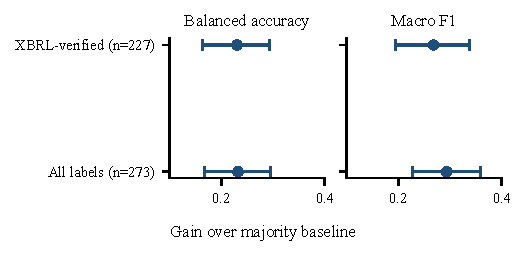
\includegraphics[width=\linewidth]{figures/effects.pdf}
\caption{Balanced-accuracy and macro-F1 gains over the majority baseline on all labels and on XBRL-verified labels. Intervals are paired bootstrap intervals over claims.}
\label{fig:effects}
\end{figure}

\subsection{Logistic decision table}
\label{app:logistic-decision}
Table~\ref{tab:logistic-decision} reports the calibrated logistic backbone at the base loss. The planner is slightly worse than always-adjudicate (3.997 versus 3.919; the fixed policy wins in 5/5 seeds). This is the strong-base-policy result discussed in Section~\ref{sec:regret-results}.

\begin{table}[t]
\centering
\small
\setlength{\tabcolsep}{3pt}
\begin{tabular}{lccc}
\toprule
Policy & Mean loss & $\Delta$ loss & Seeds \\
\midrule
Always answer & 4.712 & +.715 & 0/5 \\
Always adjudicate & 3.919 & $-.078$ & 5/5 \\
Always abstain & 5.000 & +1.003 & 0/5 \\
Planner & 3.997 & -- & -- \\
\bottomrule
\end{tabular}
\caption{Base decision loss on 227 XBRL-verified labels with the calibrated logistic backbone. Lower is better. $\Delta$ loss is the policy loss minus the planner loss. ``Seeds'' counts point estimates in which the policy has lower loss than the planner across five fold seeds.}
\label{tab:logistic-decision}
\end{table}

The logistic conformal sensitivity uses raw out-of-fold probabilities and the expected threshold objective. Averaged over five fold seeds, its base loss is 3.343, versus 3.293 for the width-tuned fixed adjudicator and 3.443 for the tuned planner. It wins under the under-averse loss (3.185 vs.\ 3.293) and the wide width penalty (4.736 vs.\ 5.508), but not at base. The realized objective is less stable on this small calibration set and is reported as an ablation in the algorithm document.

\subsection{Reproducibility}
The benchmark, planner, and figures are generated by scripts in the released repository; Appendix~\ref{app:availability} lists the data, code, prompts, and per-claim outputs. The benchmark uses fixed fold seeds and deterministic model fits. The dataset is derived from public SEC filings and XBRL, and the released JSON retains the SEC source URL for every claim. The code records the protocol constants, the feature list, the ten loss configurations, the bootstrap seeds, and the per-claim losses; it also contains the RF decision-layer run, portfolio validation selection, metric suite, named baselines, rolling benchmark, and conformal alternative. The controlled diagnostic is synthetic and is generated from fixed seeds. No online exploration is performed.

\subsection{Loss misspecification}
\label{app:cross}
The main grid optimizes and evaluates under the same loss. We also optimize the planner under one configuration and score it under another. The matched-loss mean regret is .052, and the maximum over the ten configurations is .383. When the loss is unknown, the matched planner has mean regret .821 and maximum 6.03; the .821 is the average, over the ten nominal losses, of each nominal loss's mean regret across all ten evaluation cells, including the matched cell. The strict off-diagonal mean is .906. A minimax-regret variant that chooses each action to minimize the worst-case expected regret over the ten configurations has mean .296 and maximum 2.13 across five seeds, at a cost of .296 versus .052 under the matched loss.

\begin{table}[t]
\centering
\small
\setlength{\tabcolsep}{4pt}
\begin{tabular}{lcc}
\toprule
Planner & Mean regret & Max regret \\
\midrule
Matched, known loss & .052 & .383 \\
Matched, unknown loss & .821 & 6.030 \\
Minimax regret, unknown loss & .296 & 2.130 \\
\bottomrule
\end{tabular}
\caption{Loss misspecification on XBRL-verified labels. ``Matched, known loss'' is the diagonal: optimize and evaluate under the same configuration; its maximum is over the ten configurations. ``Matched, unknown loss'' averages, for each nominal loss, the regret over all ten evaluation cells (including the matched cell); the strict off-diagonal mean is .906. The minimax maximum is the worst observed per-seed maximum.}
\label{tab:cross}
\end{table}

Per-nominal mean regret ranges from .196 (alpha=.20) to 1.863 (wide width). The full matrix is in the released artifact.

\subsection{Named baselines and rolling benchmark}
\label{app:baselines}
Table~\ref{tab:metrics} reports six named baselines adapted to the claim-outcome
task under the same DeepSeek backbone. All receive the same point-in-time
evidence; retrieval-based methods receive six earlier claims from other
companies. These are adaptations of the named methods, not official code
releases. Generic backbones are not presented as baselines. The rolling-origin
benchmark follows in Table~\ref{tab:rolling}.

\begin{table*}[t]
\centering
\small
\setlength{\tabcolsep}{3pt}
\begin{tabular}{lcccccccc}
\toprule
Model & Acc. & Bal. & Macro F1 & MCC & AUROC & AP & Sel@50 & AURC \\
\midrule
FinPlan (logistic) & .493 & .561 & .485 & .273 & .716 & .524 & .526 & .468 \\
FinDVer-style & .551 & .461 & .464 & .233 & .674 & .494 & .675 & .337 \\
Fin-Fact-style & .537 & .446 & .450 & .201 & .650 & .475 & .675 & .338 \\
Self-RAG-style & .546 & .451 & .456 & .216 & .670 & .491 & .684 & .333 \\
CRAG-style & .529 & .423 & .418 & .177 & .643 & .473 & .658 & .349 \\
FLARE-style & .511 & .417 & .411 & .164 & .634 & .467 & .596 & .362 \\
Adaptive-RAG-style & .493 & .406 & .400 & .143 & .584 & .425 & .579 & .415 \\
\bottomrule
\end{tabular}
\caption{Named baselines on 227 XBRL-verified claims. Acc.: accuracy; Bal.: balanced accuracy; MCC: Matthews correlation; AP: macro average precision; Sel@50: selective accuracy at 50\% coverage; AURC: mean risk at coverage levels .1--1.0. The six rows are prompt-level adaptations under the same DeepSeek backbone (\texttt{deepseek-flash[1m]}, temperature 0, thinking disabled), not official code releases; retrieval-based methods receive six earlier claims from other companies. The FinPlan row is the calibrated logistic evidence model; the decision portfolio uses the RF backbone. The LLM rows return a label, a confidence, and a credible set, not a normalized three-class distribution; we therefore report classification and ranking metrics only. NLL, Brier, and ECE are not comparable across these rows and are not shown. No method dominates: FinDVer has the best accuracy, Self-RAG the best selective accuracy and AURC, and FinPlan the best balanced accuracy, macro F1, MCC, AUROC, and AP. Named baselines inherit the LLM pretraining-contamination caveat. The FinPlan row pools calibrated per-claim probabilities across seeds; Table~\ref{tab:benchmark} reports a five-seed ensemble of raw probabilities, so the two balanced accuracies differ (.561 vs .564) and accuracy differs (.493 vs .517).}
\label{tab:metrics}
\end{table*}

The six rows are adaptations to this task under the same DeepSeek
backbone: FinDVer-style verification \citep{zhao2024findver}, Fin-Fact-style
evidence-grounded checking \citep{rangapur2025finfact}, Self-RAG-style
self-reflection \citep{asai2024selfrag}, CRAG-style correction
\citep{yan2024crag}, FLARE-style active retrieval \citep{jiang2023flare}, and
Adaptive-RAG-style complexity routing \citep{jeong2024adaptiverag}. Each
receives the same point-in-time evidence block: claim text, guidance range,
current-quarter value, cutoff date, sector, and the company's prior outcomes
public before the cutoff. Retrieval-based variants receive the same six
earlier claims from other companies, selected by TF-IDF cosine similarity over
claim text plus guidance-width, current-quarter-ratio, and sector features.
FinDVer, Fin-Fact, Self-RAG, and CRAG make one call. FLARE first answers
without retrieval and revises when confidence is below .70. Adaptive-RAG
routes to a simple, moderate, or complex path with a classifier prompt. All
calls use temperature 0, thinking disabled, JSON-only output, and one repair
retry; responses are cached by prompt hash. The exact prompts are in
\texttt{scripts/\allowbreak run\_named\_baselines.py}; per-claim outputs and
raw response text are in
\texttt{paper/\allowbreak results/\allowbreak named\_baselines/}.

FinDVer-style reaches accuracy .551, selective@50 .675, and AURC .337;
Self-RAG-style reaches .546, .684, and .333, the best selective accuracy and
AURC in the table. FinPlan has the best balanced accuracy .561, macro F1 .485,
MCC .273, AUROC .716, and AP .524; FinDVer-style has the best accuracy .551.
Paired McNemar tests against FinPlan do not reject equal accuracy for any named
baseline ($p=.17$--$1.00$). Fin-Fact-style, CRAG-style, FLARE-style, and
Adaptive-RAG-style have lower AUROC than FinPlan with 95\% intervals excluding
zero; the FinDVer-style and Self-RAG-style differences include zero. No point
model is uniformly best, which is why the decision layer is selected on regret
rather than on a single classification metric. Intervals are claim-level
bootstrap intervals in
\texttt{paper/\allowbreak results/\allowbreak named\_baselines/\allowbreak model\_comparison\_logistic.json};
the per-claim artifacts and the metric suite are in
\texttt{paper/\allowbreak results/\allowbreak named\_baselines/}.

\begin{table*}[t]
\centering
\small
\setlength{\tabcolsep}{3pt}
\begin{tabular}{lcccccccc}
\toprule
Model & Acc. & Bal. & Macro F1 & MCC & AUROC & AP & Sel@50 & AURC \\
\midrule
FinPlan (logistic) & .493 & .561 & .485 & .273 & .716 & .524 & .526 & .468 \\
FinDVer-style & .458 & .377 & .372 & .090 & .630 & .433 & .561 & .468 \\
Fin-Fact-style & .493 & .431 & .436 & .152 & .618 & .424 & .570 & .453 \\
Self-RAG-style & .489 & .443 & .448 & .157 & .630 & .446 & .566 & .408 \\
CRAG-style & .546 & .491 & .496 & .242 & .634 & .439 & .570 & .456 \\
FLARE-style & .476 & .380 & .376 & .097 & .595 & .408 & .553 & .466 \\
Adaptive-RAG-style & .441 & .377 & .379 & .070 & .563 & .374 & .509 & .535 \\
\bottomrule
\end{tabular}
\caption{Second backbone: the six named adaptations under GLM 5.3 flash
(\texttt{glm-5.3-flash}, reasoning effort low, temperature 0) on the same 227
verified claims. Self-RAG-style has 225 parsed claims; the other rows have 227.
FinPlan has the best balanced accuracy, macro F1, MCC, AUROC, and AP; CRAG-style
has the best accuracy; Self-RAG-style the best AURC. No point model dominates.
The GLM rows inherit the same LLM pretraining-contamination caveat.}
\label{tab:metrics-glm}
\end{table*}

On the second backbone, GLM 5.3 flash, FinPlan still has the best balanced
accuracy (.561), macro F1 (.485), MCC (.273), AUROC (.716), and AP (.524);
CRAG-style has the best accuracy (.546); Self-RAG-style has the best AURC
(.408) on 225 parsed claims. No point model dominates, and the pattern is not
specific to DeepSeek. On the 225 common claims, paired McNemar does not reject
equal accuracy for any GLM baseline ($p=.17$--$1.00$), and FinPlan's AUROC is
higher with 95\% intervals excluding zero against every GLM row. The GLM rows
are prompt-level adaptations under the same protocol, not official code
releases.


\begin{figure}[t]
\centering
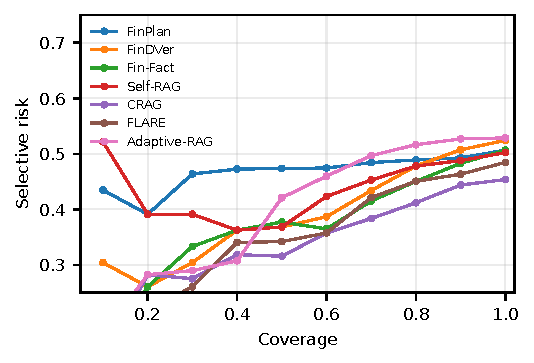
\includegraphics[width=\linewidth]{figures/risk_coverage_named.pdf}
\caption{Selective risk-coverage curves on the 227 verified claims. Self-RAG attains the lowest AURC and the highest selective accuracy among the named baselines; FinPlan has higher AURC but stronger balanced accuracy. The curves use the same per-claim probabilities as Table~\ref{tab:metrics}.}
\label{fig:risk-coverage}
\end{figure}

\begin{table}[t]
\centering
\scriptsize
\setlength{\tabcolsep}{2pt}
\begin{tabular}{lccc}
\toprule
Model & Below P/R/F1 & Within P/R/F1 & Above P/R/F1 \\
\midrule
FinPlan (logistic) & .29/.82/.43 & .63/.39/.48 & .63/.47/.54 \\
FinDVer-style & .56/.15/.24 & .46/.60/.52 & .63/.63/.63 \\
Fin-Fact-style & .50/.15/.23 & .46/.52/.49 & .60/.66/.63 \\
Self-RAG-style & .50/.15/.23 & .46/.52/.49 & .61/.68/.64 \\
CRAG-style & .43/.09/.15 & .45/.50/.47 & .59/.68/.63 \\
FLARE-style & .43/.09/.15 & .41/.56/.48 & .61/.60/.61 \\
Adaptive-RAG-style & .43/.09/.15 & .39/.57/.47 & .62/.55/.58 \\
\bottomrule
\end{tabular}
\caption{Per-class precision/recall/F1 on the 227 verified claims for the DeepSeek backbone. FinPlan has high below recall but low below precision; the named baselines miss below (recall .09--.15) and trade minority-class recall for within/above performance.}
\label{tab:per-class}
\end{table}

\begin{table}[t]
\centering
\footnotesize
\setlength{\tabcolsep}{1.5pt}
\begin{tabular}{lcccccc}
\toprule
Model & $n$ & Acc. & Bal. & F1 & ECE & Sel@50 \\
\midrule
FinPlan (RF) & 737 & .537 & .503 & .498 & .032 & .593 \\
FinPlan (logistic) & 737 & .487 & .535 & .480 & .092 & .501 \\
\bottomrule
\end{tabular}
\caption{Rolling-origin backbone check: for each cutoff year 2015--2025, train on other company folds with outcomes before January 1 and test every claim in that year. The rolling set has 737 claims and five fold seeds. The two FinPlan backbones keep the same trade-off as on the 2022--2025 test: RF has higher accuracy and lower calibration error, logistic higher balanced accuracy.}
\label{tab:rolling}
\end{table}

The rolling benchmark is a stress test, not a replacement for the main
2022--2025 holdout. It contains 737 claims from 2015--2025 (the 273 test claims
plus 464 earlier claims) and covers earlier regimes (2015--2021). The yearly
accuracy is heterogeneous (for example, logistic accuracy is .32 in 2021 and
.63 in 2024), so the aggregate is reported with the year slices in the metric
artifact rather than as a single stable number.

\paragraph{External financial RAG systems.}
FinRank \citep{mansouri2026finrank}, Fin-RATE \citep{jiang2026finrate},
HC-RAG \citep{chen2026hcrag}, and FinSAgent \citep{chi2026finsagent} are
retrieval or agent frameworks evaluated on open financial QA. We did not run
them on this decision benchmark: no compatible released code or shared claim
labels were available, and their published numbers are on different data.
Table~\ref{tab:metrics} instead adapts six general named methods under the same
base model. Those rows are adaptations, not exact reproductions of the
financial systems or of the original method code, and they are not a claim
about the published systems' relative quality.

\subsection{Real pre-hoc router}
\label{app:router}
The router is trained on validation (2019--2021) with the ex-post better mode
(answer vs adjudicate) as the label and features available at the cutoff. It
sees only features at test time; the content of the chosen mode comes from the
same logistic model. The planner in this protocol uses raw probabilities (not
the calibrated probabilities of the main table). The oracle-mode router is a
strong supervised baseline, not a strawman. At the base loss it has lower loss
than the planner (3.516 vs 3.927). Across the ten configurations the oracle-mode
router and the planner each win five: the router wins base, symmetric,
over-averse, expensive abstention, and $\alpha=.05$; the planner wins
under-averse, cheap abstention, narrow width, wide width, and $\alpha=.20$.
The width-threshold router wins five, the planner four, and narrow width is a
tie.

\begin{table*}[t]
\centering
\small
\setlength{\tabcolsep}{4pt}
\begin{tabular}{lccccc}
\toprule
Config & Width router & Oracle-mode router & Always answer & Always adjudicate & Planner \\
\midrule
base & 3.6630 & 3.5165 & 4.5128 & 3.6044 & 3.9267 \\
symmetric & 3.6996 & 3.5092 & 4.7619 & 3.6044 & 3.6557 \\
over-averse & 3.6081 & 3.5678 & 4.2857 & 3.6044 & 3.8974 \\
under-averse & 3.8828 & 3.5275 & 6.1538 & 3.6044 & 3.3114 \\
cheap abstain & 3.6630 & 3.5165 & 4.5128 & 3.6044 & 2.0513 \\
expensive abstain & 3.6630 & 3.5165 & 4.5128 & 3.6044 & 3.9267 \\
narrow width & 1.2308 & 1.5659 & 4.5128 & 1.2308 & 1.2308 \\
wide width & 5.0549 & 6.2344 & 4.5128 & 6.7692 & 4.6190 \\
alpha=.05 & 3.8535 & 3.7289 & 4.5128 & 3.8535 & 4.2637 \\
alpha=.20 & 3.3993 & 3.4799 & 4.5128 & 3.3993 & 3.4432 \\
\bottomrule
\end{tabular}
\caption{Real pre-hoc router on 273 test claims. Against the oracle-mode router
the two policies each win five of ten configurations; against the
width-threshold router the router wins five, the planner four, and one is a
tie. The planner is better when the loss makes waiting or abstention valuable;
the router is better at the base loss.}
\label{tab:router}
\end{table*}

\subsection{Controlled mode-switching diagnostic}
\label{app:controlled}
The real benchmark does not contain a strong evidence item that arrives between the cutoff and the outcome, so the planner's mode-switching behavior is tested in a controlled diagnostic. The diagnostic adds a preliminary signal available 30 days after the cutoff, at cost 0.5. Half of the cases receive a precise signal (precision .9) and half receive a weak signal (precision .5). The assignment is independent of the features a pre-hoc router can see. On the 133 cases with the precise signal, the planner acquires the signal and stops if it is informative; otherwise it waits for the final filing. A pre-hoc cost-aware router chooses wait or stop before seeing the signal.

\begin{table}[t]
\centering
\small
\setlength{\tabcolsep}{4pt}
\begin{tabular}{lcc}
\toprule
Method & Top-1 accuracy & 95\% CI \\
\midrule
Pre-hoc cost-aware router & .470 & [.458, .482] \\
Planner with preliminary & .899 & [.886, .912] \\
Paired difference & +.429 & [.411, .447] \\
\bottomrule
\end{tabular}
\caption{Controlled mode-switching diagnostic over 20 seeds, 133 cases per seed. The preliminary signal is synthetic and its assignment is independent of pre-evidence features.}
\label{tab:controlled}
\end{table}

The planner reaches top-1 accuracy .899 [.886, .912], while the pre-hoc router reaches .470 [.458, .482]. The paired difference is +.429 [.411, .447], and all 20 seeds are positive. The diagnostic isolates the mechanism in Proposition~3: the mode depends on evidence observed after the routing decision. It is not a real-data result, and we label it as controlled throughout.

\subsection{Base model and conformal alternative}
\label{app:deepseek}
DeepSeek is the shared backbone for the named baselines in
Table~\ref{tab:metrics}. The provider reports the model identifier
\texttt{deepseek-flash[1m]}; calls go through the Anthropic-compatible endpoint
with reasoning disabled, temperature 0, and JSON-only prompts. The prompt
contains the claim, the guided range, the current-quarter value, cutoff date,
sector, and the company's prior outcomes and mean surprise before the cutoff.
Responses are cached by a SHA-256 digest of the request payload; the per-claim
artifacts retain the parsed output and raw response text. The model may have
seen 2022--2025 outcomes during pretraining, so the named baselines are not
clean point-in-time evidence. The FinDVer-style and Fin-Fact-style rows replace
the earlier point/verification diagnostics; the RF-logistic comparison is a
backbone check, not a named baseline.

Replacing the planner's heuristic credible set with the loss-aware conformal
set on the same DeepSeek belief gives the result in
Table~\ref{tab:conformal}. At base the loss is 3.101, versus 3.119 for the
tuned planner; under cheap abstention it is 1.947 versus 2.511; under the wide
width penalty 4.447 versus 4.542. Base coverage is .916 with no fallback
folds. The conformal layer is not a separate reader: it consumes the same
label, confidence, and credible set as the planner.

\begin{table}[t]
\centering
\small
\setlength{\tabcolsep}{3pt}
\begin{tabular}{lccc}
\toprule
Backbone / policy & Base & Max & Wins \\
\midrule
DeepSeek + conformal & 3.101 & 4.447 & -- \\
DeepSeek + planner & 3.101 & 4.542 & 8/10 \\
Logistic + planner & 3.982 & 5.110 & 2/10 \\
DeepSeek static set & 3.154 & 5.639 & -- \\
Logistic static set & 3.877 & 7.718 & -- \\
\bottomrule
\end{tabular}
\caption{Backbone comparison on 227 verified claims. ``Max'' is the maximum
decision loss across the ten configurations. DeepSeek supplies a label,
confidence, and credible set; it is a backbone, not a separate method. The
conformal row is the five-split mean; the planner rows use the seed-1 protocol
in Appendix~\ref{app:deepseek}.}
\label{tab:backbone}
\end{table}

\subsection{Conformal alternative}
\label{app:conformal}
The conformal layer replaces the credible set by a split-conformal set
\(R_q(x)=\{y:s(x,y)\le q\}\). LAC uses \(s(x,y)=1-p(y\mid x)\); APS uses the
cumulative probability mass through \(y\). The threshold is selected on
calibration data by realized decision loss subject to empirical coverage
\(\ge 1-\alpha\); the score family and \(\alpha\) are selected on
company-disjoint validation; the threshold is recalibrated on the full
calibration set. Test outcomes are never used. The action rule is unchanged.

\begin{table}[t]
\centering
\small
\setlength{\tabcolsep}{2pt}
\begin{tabular}{lcccc}
\toprule
Backbone & Base & Cheap & Narrow & Wide \\
\midrule
DeepSeek, named & 3.101 & 1.947 & 1.053 & 4.447 \\
DeepSeek, masked company & 3.119 & 2.026 & 1.128 & 4.260 \\
\bottomrule
\end{tabular}
\caption{Conformal alternative on 227 XBRL-verified claims, five split seeds. The masked run keeps the same prompt and credible-set request but replaces company/ticker with ``Company A''. At base the named run is 3.101 versus 3.122 for the tuned fixed adjudicator; the masked run is 3.119 versus 3.108. The named result's base advantage is not robust to masking.}
\label{tab:conformal}
\end{table}

On the named DeepSeek run the conformal layer is at or below the best fixed
policy in every one of the ten loss configurations, with mean regret -0.097
and maximum -0.011. The masked run attenuates the base advantage and the cheap
abstention advantage (2.026 versus always-abstain 2.000), so we do not treat
the LLM result as clean point-in-time evidence. On the RF backbone the
conformal layer is worse than the planner (mean regret +0.047, maximum +0.148).
The conformal layer is therefore an alternative set constructor, not the
selected primary method.


\subsection{Real sequential evidence}
\label{app:sequential}
The dataset's outcome date is the 10-Q filing date, but for 993 of 1,005
claims the same quarter's revenue was public earlier in an 8-K Item 2.02
earnings release (median 2 days earlier; all 273 test claims have one). The
sequential experiment uses that release as the real terminal evidence. At the
cutoff the agent may stop with answer, adjudicate, or abstain; acquire the next
peer company's outcome at cost $.1$ or $.5$; or wait for the earnings release
at cost $2.0$ plus $\gamma$ per day. The belief is a snapshot logistic model
trained on 2010--2020 claims with target features, peer summary, and days since
cutoff; 2021 is validation; the 227 verified 2022--2025 claims are test. The
portfolio starts from fixed adjudication and switches only when a candidate
improves validation loss by $.1$. Across 24 cost cells (six $\gamma$, two
evidence costs, two outcome costs), the portfolio matches the best candidate in
every cell (mean and maximum regret 0); it selects always-wait in the eight
cheap-delay cells and fixed adjudication in the sixteen expensive cells. The
planner with peer acquisition is never selected; peer evidence is too weak
relative to its cost. The result is a decision-time selection result, not a
planner-superiority result.

\begin{table}[t]
\centering
\small
\setlength{\tabcolsep}{3pt}
\begin{tabular}{lcccc}
\toprule
$\gamma$ & Fixed adj. & Always wait & Planner & Selected \\
\midrule
0.00 & 3.912 & 2.000 & 2.318 & wait \\
0.01 & 3.912 & 2.827 & 3.378 & wait \\
0.02 & 3.912 & 3.653 & 4.521 & wait \\
0.05 & 3.912 & 6.133 & 4.588 & fixed \\
\bottomrule
\end{tabular}
\caption{Real sequential evidence on 227 verified test claims (evidence cost
$.1$, outcome cost $2.0$). ``Planner'' is the one-step lookahead with peer
acquisition and a $.2$ conservative margin. The portfolio selects wait when
delay is cheap and fixed adjudication when it is expensive; it matches the
oracle best candidate in all 24 cost cells.}
\label{tab:sequential}
\end{table}


\end{document}
